\chapter{DISCRETIZAÇÃO}
A estimação de densidade via \ac{KDE} de uma série de medidas contínuas, por razões computacionais, é geralmente representado na forma discreta. Consequentemente, estimações diretas acontecem apenas para valores discretizados \cite{jones1989discretized} e interpolação é usado para solucionar qualquer outro valor que possa vir fora durante as mediações. Este processo insere erros de estimação os quais podem ser minimizados incrementando o número de pontos a serem estimados, buscando um equilíbrio entre otimização computacional e performance de estimação.

Vários autores seguem a mesma abordagem, como em \cite{jones1989discretized}, explorando os diferentes aspectos do processo de discretização e propondo novos métodos no intuito de minimizar as adversidades relatadas. Por exemplo, em \cite{fayyad1993multi} o método bem conhecido Ent-MDLP é proposto; em \cite{friedman1996discretizing} é sugerido um algoritmo de discretização baseado em Redes Bayesianas; em \cite{biba2007unsupervised} os autores propõem um método não supervisionado para discretização utilizando-se o \ac{KDE}; também usando o método não supervisionado, os autores de \cite{schmidberger2005unsupervised} apresentam um estudo de discretização aplicado à estimação de densidade baseado em árvore; e em \cite{zhang2007discretization} um algoritmo de aprendizagem de máquina baseado-se no critério de \textit{Gini} foi estudado. 

Estes trabalhos geralmente possuem foco em algoritmos de aprendizagem de máquina ou minimização dos critérios selecionados a fim de otimizar os vários atributos existentes, que como consequência, tendem a ter um alto custo computacional quando submetidos a uma grande quantidade de dados. Além do mais, tais estudos abordam a performance da discretização através do prisma da classificação e alguns como forma de preprocessamento do conjunto de dados.

O método de discretização mais aplicado atualmente é o baseado em espaçamento uniforme entre os pontos estimados. Isso trata de maneira igualitária todas as densidades de região (e. g. a função de densidade nas regiões de baixa probabilidade é discretizada com a mesma resolução das regiões de alta probabilidade) levando a um erro de estimação que tende a não ser uniforme ao longo de todas as regiões de função de densidade de probabilidade.
A figura~\ref{fig:figura1} mostra um exemplo de quando a região de baixa probabilidade é grande devido a eventos fora da curva, neste caso, uma discretização baseada em um espaçamento uniforme  pode colocar um grande número de pontos desnecessários nessa região, fazendo com que, para minimizar o erro de estimação, o número de pontos a ser estimado seja maior a fim de representar bem a região de alta probabilidade. %enquanto regiões de alta probabilidade terão que usar mais pontos a fim de minimizar o erro de estimação.

\begin{figure}[H]
	\centering
	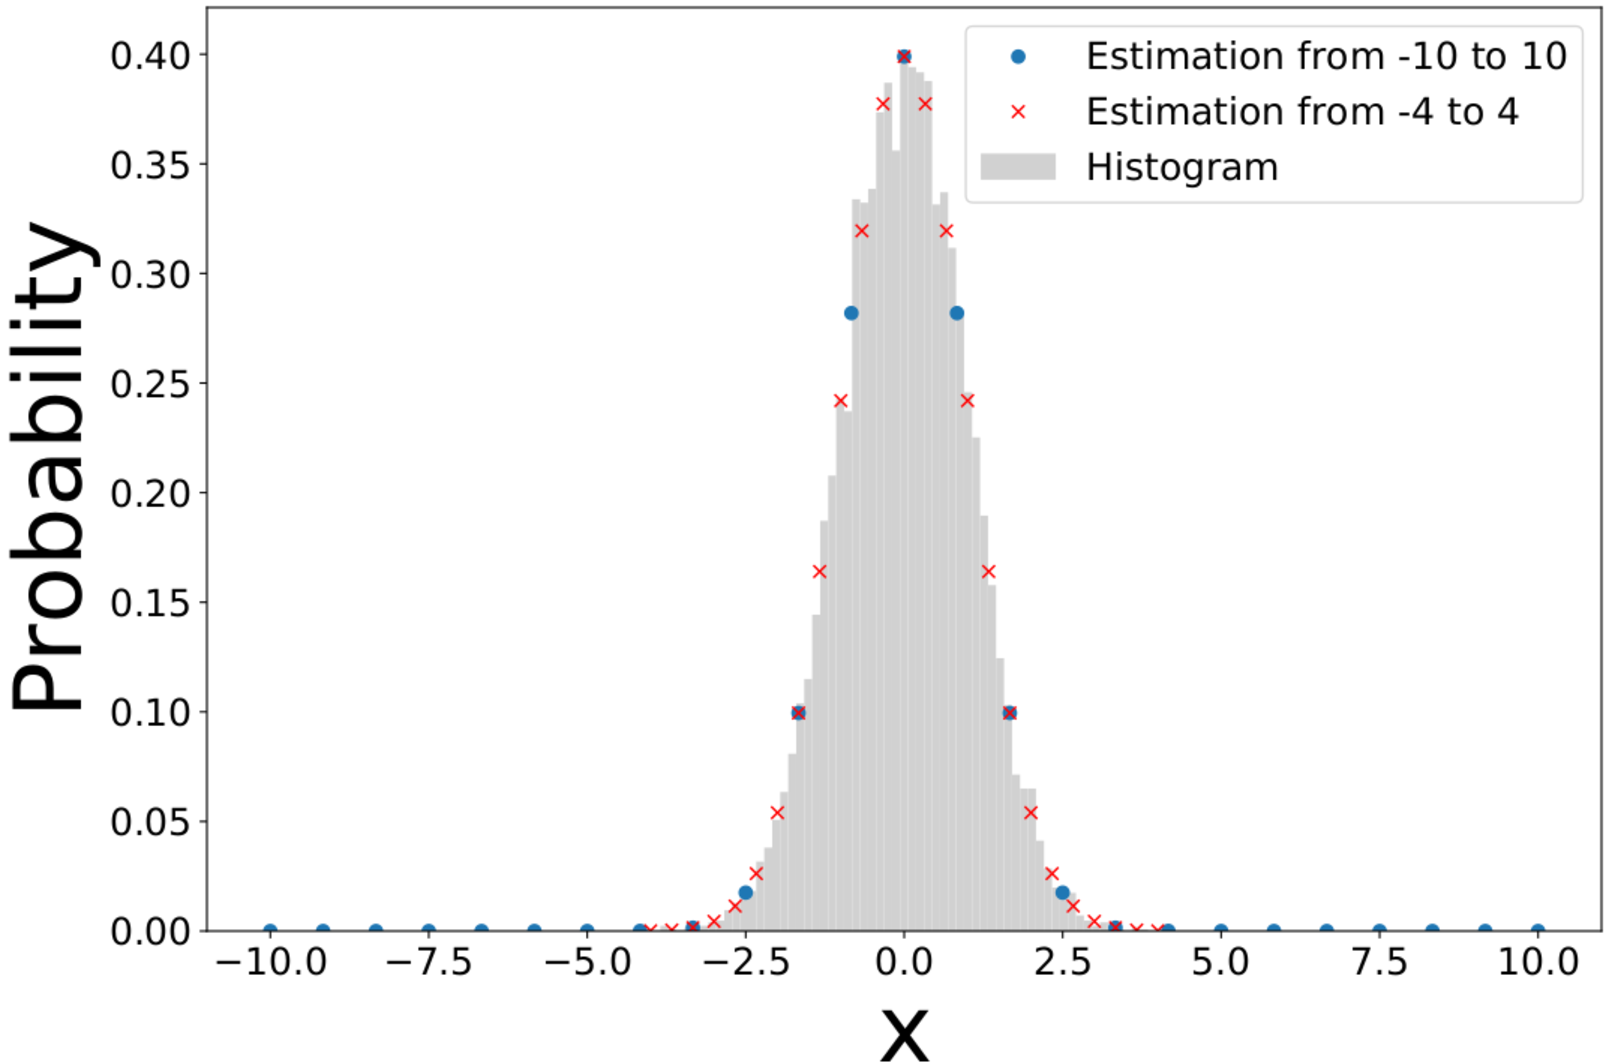
\includegraphics[width=0.6\linewidth]{figuras/linspace2}
	\caption{Caso representativo de estimação de PDF utilizando 25 pontos para dois intervalos diferentes (-4,4) e (-10,10)}
	\label{fig:figura1}
\end{figure}